\documentclass[journal,12pt,twocolumn]{IEEEtran}

\usepackage{setspace}
\usepackage{gensymb}
\singlespacing
\usepackage[cmex10]{amsmath}
\usepackage{caption}

\usepackage{amsthm}

\usepackage{mathrsfs}
\usepackage{txfonts}
\usepackage{stfloats}
\usepackage{bm}
\usepackage{cite}
\usepackage{cases}
\usepackage{subfig}

\usepackage{longtable}
\usepackage{multirow}

\usepackage{enumitem}
\usepackage{mathtools}
\usepackage{steinmetz}
\usepackage{tikz}
\usepackage{circuitikz}
\usepackage{verbatim}
\usepackage{tfrupee}
\usepackage[breaklinks=true]{hyperref}
\usepackage{graphicx}
\usepackage{tkz-euclide}

\usetikzlibrary{calc,math}
\usepackage{listings}
    \usepackage{color}                                            %%
    \usepackage{array}                                            %%
    \usepackage{longtable}                                        %%
    \usepackage{calc}                                             %%
    \usepackage{multirow}                                         %%
    \usepackage{hhline}                                           %%
    \usepackage{ifthen}                                           %%
    \usepackage{lscape}     
\usepackage{multicol}
\usepackage{chngcntr}

\DeclareMathOperator*{\Res}{Res}

\renewcommand\thesection{\arabic{section}}
\renewcommand\thesubsection{\thesection.\arabic{subsection}}
\renewcommand\thesubsubsection{\thesubsection.\arabic{subsubsection}}

\renewcommand\thesectiondis{\arabic{section}}
\renewcommand\thesubsectiondis{\thesectiondis.\arabic{subsection}}
\renewcommand\thesubsubsectiondis{\thesubsectiondis.\arabic{subsubsection}}


\hyphenation{op-tical net-works semi-conduc-tor}
\def\inputGnumericTable{}                                 %%

\lstset{
%language=C,
frame=single, 
breaklines=true,
columns=fullflexible
}
\begin{document}


\newtheorem{theorem}{Theorem}[section]
\newtheorem{problem}{Problem}
\newtheorem{proposition}{Proposition}[section]
\newtheorem{lemma}{Lemma}[section]
\newtheorem{corollary}[theorem]{Corollary}
\newtheorem{example}{Example}[section]
\newtheorem{definition}[problem]{Definition}

\newcommand{\BEQA}{\begin{eqnarray}}
\newcommand{\EEQA}{\end{eqnarray}}
\newcommand{\define}{\stackrel{\triangle}{=}}
\bibliographystyle{IEEEtran}
\raggedbottom
\setlength{\parindent}{0pt}
\providecommand{\mbf}{\mathbf}
\providecommand{\pr}[1]{\ensuremath{\Pr\left(#1\right)}}
\providecommand{\qfunc}[1]{\ensuremath{Q\left(#1\right)}}
\providecommand{\sbrak}[1]{\ensuremath{{}\left[#1\right]}}
\providecommand{\lsbrak}[1]{\ensuremath{{}\left[#1\right.}}
\providecommand{\rsbrak}[1]{\ensuremath{{}\left.#1\right]}}
\providecommand{\brak}[1]{\ensuremath{\left(#1\right)}}
\providecommand{\lbrak}[1]{\ensuremath{\left(#1\right.}}
\providecommand{\rbrak}[1]{\ensuremath{\left.#1\right)}}
\providecommand{\cbrak}[1]{\ensuremath{\left\{#1\right\}}}
\providecommand{\lcbrak}[1]{\ensuremath{\left\{#1\right.}}
\providecommand{\rcbrak}[1]{\ensuremath{\left.#1\right\}}}
\theoremstyle{remark}
\newtheorem{rem}{Remark}
\newcommand{\sgn}{\mathop{\mathrm{sgn}}}
\providecommand{\abs}[1]{\left\vert#1\right\vert}
\providecommand{\res}[1]{\Res\displaylimits_{#1}} 
\providecommand{\norm}[1]{\left\lVert#1\right\rVert}
%\providecommand{\norm}[1]{\lVert#1\rVert}
\providecommand{\mtx}[1]{\mathbf{#1}}
\providecommand{\mean}[1]{E\left[ #1 \right]}
\providecommand{\fourier}{\overset{\mathcal{F}}{ \rightleftharpoons}}
%\providecommand{\hilbert}{\overset{\mathcal{H}}{ \rightleftharpoons}}
\providecommand{\system}{\overset{\mathcal{H}}{ \longleftrightarrow}}
 %\newcommand{\solution}[2]{\textbf{Solution:}{#1}}
\newcommand{\solution}{\noindent \textbf{Solution: }}
\newcommand{\cosec}{\,\text{cosec}\,}
\providecommand{\dec}[2]{\ensuremath{\overset{#1}{\underset{#2}{\gtrless}}}}
\newcommand{\myvec}[1]{\ensuremath{\begin{pmatrix}#1\end{pmatrix}}}
\newcommand{\mydet}[1]{\ensuremath{\begin{vmatrix}#1\end{vmatrix}}}
\numberwithin{equation}{subsection}
\makeatletter
\@addtoreset{figure}{problem}
\makeatother
\let\StandardTheFigure\thefigure
\let\vec\mathbf
\renewcommand{\thefigure}{\theproblem}
\def\putbox#1#2#3{\makebox[0in][l]{\makeb
ox[#1][l]{}\raisebox{\baselineskip}[0in][0in]{\raisebox{#2}[0in][0in]{#3}}}}
     \def\rightbox#1{\makebox[0in][r]{#1}}
     \def\centbox#1{\makebox[0in]{#1}}
     \def\topbox#1{\raisebox{-\baselineskip}[0in][0in]{#1}}
     \def\midbox#1{\raisebox{-0.5\baselineskip}[0in][0in]{#1}}
\vspace{3cm}
\title{Assignment 2}
\author{Tarandeep Singh}
\maketitle
\newpage
\bigskip
\renewcommand{\thefigure}{\theenumi}
\renewcommand{\thetable}{\theenumi}
Github Link
\begin{lstlisting}
https://github.com/Tarandeep97/AI5030
\end{lstlisting}
\section{Problem}
(52) Suppose X$\sim$ Cauchy(0,1). Then the distribution of
$\frac{1-X}{1+X}$ is?
\section{Solution - Method I}
A continuous random variable X follows \textbf{Cauchy distribution} with parameters $\mu$ and $\lambda$ if its pdf is given by
\\
    \begin{equation*} f(x) =\left\{ \begin{array}{ll} \frac{\lambda}{\pi}\cdot \frac{1}{\lambda^2+(x-\mu)^2}, & \hbox{$-\infty < x< \infty$;} \\ & \hbox{$-\infty < \mu< \infty$, $\lambda>0$;} \\ 0, & \hbox{Otherwise.} \end{array} \right. \end{equation*}
    
\\
The parameter $\mu$ and $\lambda$ are location and scale parameters respectively. 
\\
When $\mu$=0 and $\lambda$=1, then the distribution is called \textbf{Standard Cauchy Distribution}. The pdf of standard Cauchy distribution is
\\
\begin{equation*} f(x) =\left\{ \begin{array}{ll} \frac{1}{\pi}\cdot \frac{1}{1+x^2}, & \hbox{$-\infty < x< \infty$;} \\ 0, & \hbox{Otherwise.} \end{array} \right. \end{equation*}

Let,
\begin{align}
    Y = g(X) = \frac{1-X}{1+X}
\end{align}
\textbf{Range of Y} \\
Since g(X) is self-inverse of itself,it is bijective in nature. Self-inverse nature of g(X) is verified below,
\begin{align}
    g\left(\frac{1-X}{1+X}\right) = \frac{1-\frac{1-X}{1+X}}{1+\frac{1-X}{1+X}}
    = X
\end{align}
So, g(X) $\in (-\infty,\infty)$. \\
\\

\textbf{Expression for CDF of Y}
\begin{align}
    F_{Y}(y) = P(Y \leq y)
\end{align}
\begin{align}
    = P\left(\frac{1-X}{1+X} \leq y\right)
\end{align}
If X $\in (-\infty,-1)$, $(1+X)<0$. So, inequality should be reversed.
\begin{align}
    = P\left((1-X) \geq y.(1+X)\right)
\end{align}
\begin{align}
    = P\left((1-X) \geq (y+y.X)\right)
\end{align}
\begin{align}
    = P\left((1-y) \geq (X+y.X)\right)
\end{align}

\begin{align}
    = P\left(\frac{1-y}{1+y} \geq X \right) = P\left[-\infty < X \leq \left(\frac{1-y}{1+y}\right)\right]
\end{align}
\begin{align}
    = F_{X}\left(\frac{1-y}{1+y}\right) - F_{X}(-\infty)
\end{align}
If X $\in (-1,\infty)$, $(1+X)>0$. The expression can be rewritten as
\begin{align}
    = P\left(\frac{1-y}{1+y} \leq X \right)
\end{align}
\begin{align}
    = P\left[\left(\frac{1-y}{1+y}\right) \leq X < \infty \right]
\end{align}
\begin{align}
    = F_{X}(\infty) - F_{X}\left(\frac{1-y}{1+y}\right)
\end{align}
Now, using above equation CDF of Y will be,
\begin{align}
   F_{Y}(y) = P\left[-\infty < X \leq -1 \right] + P\left[\left(\frac{1-y}{1+y}\right) \leq X < \infty \right]
\end{align}
\begin{align}
    = \left(F_{X}(-1) - F_{X}(-\infty)\right) + \left(F_{X}(\infty) - F_{X}\left(\frac{1-y}{1+y}\right)\right)
\end{align}
\begin{align}
    = \frac{3}{4}-\frac{1}{\pi}.tan^{-1}\left(\frac{1-y}{1+y}\right)\right)
\end{align}
\textbf{Expression for PDF of Y}
\begin{align}
    f_{Y}(y) = \frac{d F_{Y}(y)}{dy} = -\frac{1}{\pi}\cdot\frac{d\left(tan^{-1}\left({\frac{1-y}{1+y}}\right)\right)}{dy}
\end{align}
\begin{align}
    = -\frac{1}{\pi}\cdot\frac{1}{1+\left(\frac{1-y}{1+y}\right)^{2}}\cdot\frac{d\left({\frac{1-y}{1+y}}\right)}{dy}
\end{align}
\begin{align}
    = -\frac{1}{\pi}\cdot\frac{1}{1+\left(\frac{1-y}{1+y}\right)^{2}}\cdot\left( -\frac{2}{\left(y + 1\right)^{2}}\right)
\end{align}
\begin{align}
    = \frac{1}{\pi}\cdot \frac{1}{1+y^2}
\end{align}
Hence,  Y $\sim$ Cauchy(0,1).\\
\section{Solution - Method II}
\textbf{Theorem}: If U$\sim$ Normal(0,1),V$\sim$ Normal(0,1) are independent then $X = \frac{U}{V}$ is a Cauchy Distribution.
\begin{align}
    Y = \frac{1-X}{1+X} = \frac{1-\frac{U}{V}}{1+\frac{U}{V}} = \frac{U-V}{U+V} 
\end{align}
U-V and U+V are also independent and normally distributed. \\
Hence, Y$\sim$Cauchy(0,1).
\section{Appendix}
\textbf{Theorem}: If U$\sim$ Normal(0,1),V$\sim$ Normal(0,1) are independent then $X = \frac{U}{V}$ is a Cauchy Distribution. \\ 
\\
\textbf{Proof}:
PDF of U and V is given as,
\begin{align}
    f_{U}(u) = \frac{1}{\sqrt{2\pi}}.e^{-\frac{u^{2}}{2}},f_{V}(v) = \frac{1}{\sqrt{2\pi}}.e^{-\frac{v^{2}}{2}}
\end{align}
where $-\infty<$u,v $<\infty$ \\
Since U and V are independent, their joint PDF is given by,
\begin{align}
    f_{UV}(u,v) = \frac{1}{2\pi}.e^{-\frac{u^{2}+v^{2}}{2}}
\end{align}
\begin{align}
    F_{X}(x) = P(X\leq x) = P\left(\frac{U}{V}\leq x\right)
\end{align}
\begin{align}
     = P(U\leq V.x,V\geq 0)+P(U\geq V.x,V< 0)
\end{align}
\begin{align}
     = \int_{0}^{\infty} \int_{-\infty}^{v.x} f_{uv}(u,v) \,du \,dv + \int_{-\infty}^{0} \int_{-\infty}^{v.x} f_{uv}(u,v) \,du \,dv
\end{align}
Differentiating $F_{X}(x)$ to obtain PDF of X, $f_{X}(x)$ \\
(Using Leibniz's Integral Rule)
\begin{align}
    f_{X}(x) = \int_{0}^{\infty} v. f_{uv}(vx,v) \,dv + \int_{-\infty}^{0}(-v).f_{uv}(vx,v) \,dv
\end{align}
\begin{align}
    f_{X}(x) = \int_{0}^{\infty} v. \frac{1}{2\pi}.e^{-\frac{(1+x^{2})v^{2}}{2}} \,dv + \int_{-\infty}^{0}(-v).\frac{1}{2\pi}.e^{-\frac{(1+x^{2})v^{2}}{2}}\,dv
\end{align}
Let,
\begin{align}
 u = \frac{(1+x^2)v^2}{2}
\end{align}
\begin{align}
 \frac{du}{dv} = (1+x^2)v \Rightarrow dv = \frac{du}{(1+x^2)v}
\end{align}
\begin{align}
    f_{X}(x) = \int_{0}^{\infty}  \frac{1}{2\pi (1+x^2)}.e^{-u} \,du - \int_{-\infty}^{0}\frac{1}{2\pi(1+x^2)}.e^{-u}\,du
\end{align}
\begin{align}
    f_{X}(x) = \frac{1}{\pi(1+x^2)}
\end{align}
Hence, X$\sim$ Cauchy(0,1) \\
\textbf{Theorem}: If U$\sim$ Normal(0,1) and V$\sim$ Normal(0,1), then (U-V) and (U+V) are independent. \\
\textbf{Proof}: For (U+V) and (U-V) to be independent their co-variance must be 0.
\begin{align}
   = E[(U+V)(U-V)]-E[U+V]E[U-V]
\end{align}
\begin{align}
   = E[U^2]+E[V^2]-(E[U]+E[V])(E[U]-E[V])
\end{align}
Hence,
\begin{align}
   cov(U+V,U-V)=0
\end{align}
\textbf{Leibniz Integral Rule:}
For an integral form \[ \int_{a(x)}^{b(x)} f(x,t) \,dt \]
where $-\infty<a(x),b(x)<\infty$, the derivative of this integral is expressed as,
\begin{align}
   \frac{d}{dx} \left(\int_{a(x)}^{b(x)} f(x,t) \,dt\right)
\end{align}
\begin{align}
   = f(x,b(x)).\frac{d}{dx}b(x)-f(x,a(x)).\frac{d}{dx}a(x) \\
   +\int_{a(x)}^{b(x)} \frac{\partial}{\partial x} f(x,t) \,dt
\end{align}
\begin{figure}[ht]
\centering
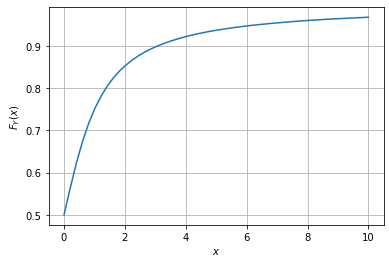
\includegraphics[width=\columnwidth]{cdf.png}
\caption*{Fig 1. CDF of Y}
\label{fig:fig1}
\end{figure}
\begin{figure}[ht]
\centering
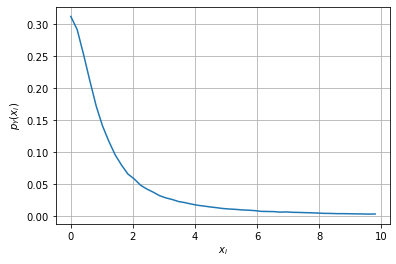
\includegraphics[width=\columnwidth]{pdf.png}
\caption*{Fig 2. PDF of Y}
\label{fig:fig2}
\end{figure}

\end{document}
